\graphicspath{{./figures}}

\section{Component Selection}
The first step in the detailed design process is to select components for the various sub-systems. Components for both the ground station and PQ unit will be selected in one step, as there is little reason to separate the two process. Ideally, components should be readily available from local suppliers.

\subsection{Existing Components}
The ground station has a number components which will be used without modification. Two \textit{NEMA 17 4218S-15} stepper motors will be used to ultimately steer the ground station (i.e. in elevation and azimuthal directions as shown in Figure \ref{fig:az_elevation}). These motors draw 0.50 A and allow for up to $\SI{0.5}{N \cdot m}$ of torque \cite{datasheet-4118}.

The ground station also includes a small zero-sensing circuit for the azimuthal direction, which integrates a \textit{H22A} optical switch \cite{datasheet-H22A1} and a low-pass filter.

\begin{figure}[!htb]
    \centering
    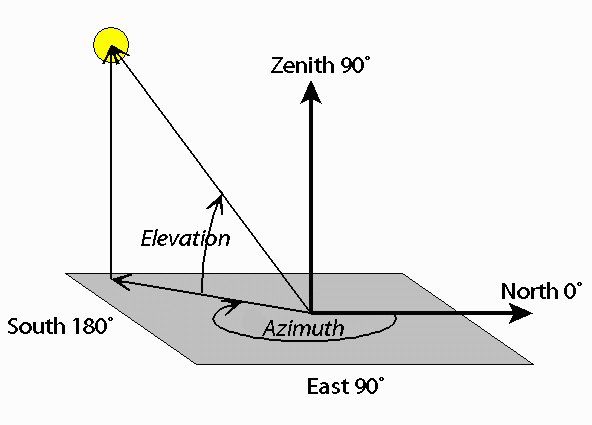
\includegraphics[width=0.4\textwidth]{az_elevation}
    \caption{Azimuthal and Elevation Visualization \cite{site-azElevationVisual}}
    \label{fig:az_elevation}
  \end{figure}

\subsection{GPS}\label{sec:components_gps}
A GPS should be selected for the ground station, and possibly for the PQ unit. In order to cater for Phase 2, and for simplified system development, a GPS module will be chosen that is suitable for both the PQ unit and the GS. To estimate GPS accuracy, a 1 degree variation is used (since the beamwidth of a typical antenna is an order of magnitude larger). A distance of \SI{100}{km} therefore results in a required accuracy of $2 \times 100 000 \times \pi \times \frac{1}{360} \approx \SI{2}{km}$, which is very large.

The NEO line of GPS modules from \textit{u-blox} are very commonly used, and are quoted to have a 2.5 m accuracy, however there was limited availability of these modules from local supplies (e.g. the \textit{NEO-6M}). Modules with similiar specifications from \textit{Makerbase} were therefore considered, such as the \textit{ATGM336H} and the \textit{ATGM332D}. Since both of these advertise 2.5 m accuracy, active antenna support, and current consumption less than 100 mA, the ATGM332D-5N31 was chosen for its lower price.

\subsection{IMU}
Generally, the ground station's orientation can be described by azimuthal and elevation angles as in Figure \ref{fig:az_elevation}. The ground station requires absolute azimuth angle measurement data, as well as elevation angle/tilt data, in order to orientate itself with respect to its surroundings. To determine absolute azimuthal rotation, the ground station should either be manually positioned to face north, or a magnetometer can be used. An accelerometer can be used to determine tilt rotation.

The above sensors, as well as a gyroscope, are typically packaged into an \textit{intertial measurement unit} (IMU). As seen in Section \ref{sec:components_gps}, only very primitive, low accuracy is required. \textit{Sensor fusion} is the mathematical process of converting raw sensor data into meaningful orientation angles. This is critical for fast-moving systems, where the accelerometer suffers during fast movements, and the gyroscope suffers due to noise drift over time.

The \textit{BNO055} is a 9-axis IMU which integrates an ARM Cortex-M0 to perform sensor fusion. It operates at 100 Hz, has $\SI{0.3}{\micro T}$ magnetic field resolution, and around 16 bit sensors. It, however, is very expensive (around R800). The \textit{MPU-9250}, and the \textit{MPU} line of IMU's in general, are seen as cheaper alternatives. Since the grouond station will be moving slowly, there is low requirement for complex sensor fusion algorithms. Since the MPU also has a 16-bit accelerometer, and only slightly lower magnetic field accuracy (\SI{0.6}{\micro T}), but is only around R150, it was selected.
